\documentclass[t]{beamer}

\usepackage{wrapfig}
\usepackage{float}
% For tabs in verbatim
\usepackage{fancyvrb}

% set fonts
\usefonttheme{professionalfonts} % using non standard fonts for beamer
\usepackage{txfonts,mathptmx}

% set indend spacing for first and second level indentation
\setlength{\leftmargini}{0.5cm}
\setlength{\leftmarginii}{0.5cm}

% Set circles for bullets 
\setbeamertemplate{itemize items}[circle]

% todo lists
\usepackage{pifont}
\usepackage{amssymb}

% increase space between text and frame name
\addtobeamertemplate{frametitle}{}{\vspace{1em}}

%Information to be included in the title page:
\title{Describing Verilog Applications}
\author{Nikola Petrovic}
\institute{University of Belgrade, School of Electrical Engineering}
\date{2022}



\begin{document}

\frame{\titlepage}

%%%%%%%%%%%%%%%%%%%%%%%%%%%%%%%%%%%%%%%%%%%%%%%%%%%%%%%%%%%%
\begin{frame}
\frametitle{Module Objective}

We well explain the nature and use of Hardware Description Language (HDL)
\newline

\textbf{Topics}

\begin{itemize}
\item What the heck is an HDL?
\item levels of abstraction
\item What are the benefits of using HDLs, we do we care?
\item The Verilog HDL
\end{itemize}

\end{frame}


%%%%%%%%%%%%%%%%%%%%%%%%%%%%%%%%%%%%%%%%%%%%%%%%%%%%%%%%%%%%
\begin{frame}
\frametitle{Terms and Definitions}

Hardware Description Language (HDL)
\begin{itemize}
\item A programming-like language that describes the functionality of digital electronic hardware circuits
\end{itemize}
Simulator:
\begin{itemize}
\item Software that imitates the functionality of electronic hardware as described by the HDL
\end{itemize}
Level of Abstraction:
\begin{itemize}
\item The level of detail provided by the utilized modeling style, such as behavioral and gate-level
\end{itemize}
Application Specific Integrated Circuit (ASIC):
\begin{itemize}
\item Integrated circuit developed for specific application
\end{itemize}
\end{frame}

%%%%%%%%%%%%%%%%%%%%%%%%%%%%%%%%%%%%%%%%%%%%%%%%%%%%%%%%%%%%
\begin{frame}
\frametitle{Terms and Definitions Continued}

Bottom-Up Design Flow:
\begin{itemize}
\item A design methodology in which you build the low-level components first and then connect them to make large systems
\end{itemize}
Top-Down Design Flow:
\begin{itemize}
\item A design methodology in which you define the system at the very high level of abstraction and then iteratively refine it
\end{itemize}
Register Transfer Level (RTL):
\begin{itemize}
\item A level of abstraction that defines storage elements and their clocks
\end{itemize}
Tool Command Language (TCL):
\begin{itemize}
\item A scripting language used for issuing commands to interactive programs
\end{itemize}
\end{frame}

%%%%%%%%%%%%%%%%%%%%%%%%%%%%%%%%%%%%%%%%%%%%%%%%%%%%%%%%%%%%
\begin{frame}
\frametitle{What is HDL}

A HDL is a programming language with special constructs for Modeling hardware concurrency and timing.
\newline

A HDL supports design at multiple levels of abstraction:
\begin{wrapfigure}{r}{0.4\textwidth}
  \begin{figure}[H!]
    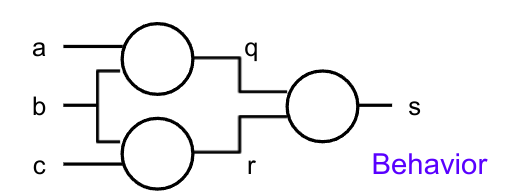
\includegraphics[width=0.38\textwidth]{img/01_beh.png}
    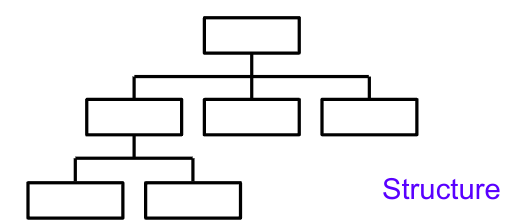
\includegraphics[width=0.38\textwidth]{img/01_struct.png}
    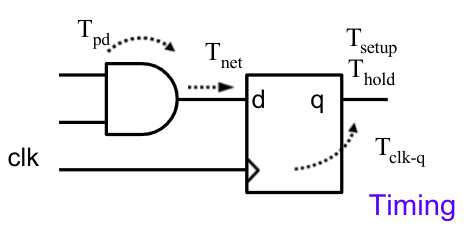
\includegraphics[width=0.38\textwidth]{img/01_tim.png}
  \end{figure}
\end{wrapfigure}
\textcolor{blue}{Behavioral Modeling:}
\begin{itemize}
\item Sequential behaviours
\item Parallel behaviours
\end{itemize}

\textcolor{blue}{Structural Modeling}:
\begin{itemize}
\item Hardware component hierarchy
\item Software subroutine hierarchy
\end{itemize}

An HDL typically supports simulation of estimated design timing.
\end{frame}



%%%%%%%%%%%%%%%%%%%%%%%%%%%%%%%%%%%%%%%%%%%%%%%%%%%%%%%%%%%%
\begin{frame}
\frametitle{HDL levels of abstraction and trade-offs}

\textcolor{blue}{Behavioral Level}:
\begin{itemize}
\item Algorithms
\end{itemize}

\textcolor{blue}{Register Transfer level (RTL)}:
\begin{itemize}
\item Mets and Registers
\end{itemize}

\textcolor{blue}{Gate Level}:
\begin{itemize}
\item Built-in \& user-defined primitives
\end{itemize}

\textcolor{blue}{Switch Level}:
\begin{itemize}
\item Built-in switch primitives
\end{itemize}

\vspace{12pt}
Simulation effort is proportional to details.
\end{frame}

%%%%%%%%%%%%%%%%%%%%%%%%%%%%%%%%%%%%%%%%%%%%%%%%%%%%%%%%%%%%
\begin{frame}[fragile]
\frametitle{Abstraction Level Example: Divide by 2}

\textcolor{blue}{BEHAVIORAL}
\begin{Verbatim}[tabsize=4]
always @(din)
	dout = din/2;
\end{Verbatim}

\textcolor{blue}{RTL}
\begin{Verbatim}[tabsize=4]
always @(posedge clk)
	dout <= din >> 1;
\end{Verbatim}

\textcolor{blue}{STRUCTURAL}
\begin{Verbatim}[tabsize=4]
FD1 op[3:0] (
	.D({1'b0, din[3:1]}),
	.CP(clk),
	.Q(dout)
);
\end{Verbatim}
\end{frame}


%%%%%%%%%%%%%%%%%%%%%%%%%%%%%%%%%%%%%%%%%%%%%%%%%%%%%%%%%%%%
\begin{frame}
\frametitle{Why should we care about HDL?}

The benefits of using HDL are:
\newline

\begin{itemize}
\item We write HDL in simple ASCII text
\begin{itemize}
	\item Capture the design quickly and easily manage modifications
\end{itemize}
\item We can design at higher abstraction level
\begin{itemize}
	\item Easily explore design alternatives
	\item Find problems earlier in design cycle
\end{itemize}
\item HDL enables design reuse
\begin{itemize}
	\item Between teams or through the design flow
	\item No re-entry, reformatting, or translation
\end{itemize}
\item HDL code is independent of the implementation
\begin{itemize}
	\item We can delay the choice of implementation technology
	\item We can more easily make architectural and functional changes
	\item We can more easily adapt our design to the future projects
\end{itemize}
\end{itemize}

\end{frame}

%%%%%%%%%%%%%%%%%%%%%%%%%%%%%%%%%%%%%%%%%%%%%%%%%%%%%%%%%%%%
\begin{frame}
\frametitle{HDL-Based Simulations}

\begin{figure}[H!]
    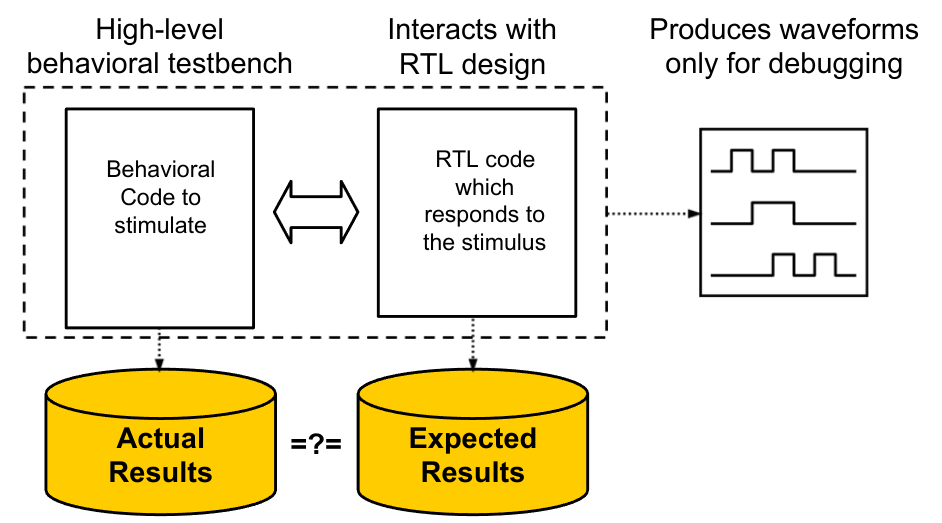
\includegraphics[width=0.98\textwidth]{img/01_sim.png}
\end{figure}

\textcolor{red}*Testbench can be self-checking.


\end{frame}


%%%%%%%%%%%%%%%%%%%%%%%%%%%%%%%%%%%%%%%%%%%%%%%%%%%%%%%%%%%%
\begin{frame}
\frametitle{HDL Adoption Issues}

What Issues we can expect in using HDLs:
\begin{itemize}
\item Well, one more thing to learn!
\begin{itemize}
	\item A new programming language to overcome
	\item Simulation and synthesis EDA tools to learn
\end{itemize}
\item Major change in design methodology
\begin{itemize}
	\item No standard "off the shelf methodology"
	\item Needs to be planned and implemented
\end{itemize}
\item Primarly targets digital design
\begin{itemize}
	\item Analog extensions exists, but we will pretend that they don't
\end{itemize}
\item Design planning and partitioning required before coding
\item Coding style influences project time-to-closure
\item Other specific issues that we will see during this course
\end{itemize}
\end{frame}

%%%%%%%%%%%%%%%%%%%%%%%%%%%%%%%%%%%%%%%%%%%%%%%%%%%%%%%%%%%%
\begin{frame}
\frametitle{The Verilog}

In this course we well focus on Verilog, VHDL you have probably learned in school.
\newline

\begin{itemize}
\item Developed in 1983 by Phil Moorby and Prabhu Goel at Automated Integrated Design Systems (don't read the acronym)
\item Syntax: Kinda like C
\item Paradigm: Procedural assignment of values to variables
\item Types: Loosely typed Language
\item Comprehensive language with no facility for user extensions
\end{itemize}
\end{frame}

%%%%%%%%%%%%%%%%%%%%%%%%%%%%%%%%%%%%%%%%%%%%%%%%%%%%%%%%%%%%
\begin{frame}
\frametitle{Verilog Language Versions}

The IEEE Std 1364-2005 had relatively few major extensions over Verilog-2001.
\newline

As of 2009, the SystemVerilog and Verilog language standards were merged into SystemVerilog 2009 (IEEE Std 1800-2009). The current version is IEEE Std 1800-2017.

\begin{figure}[H!]
    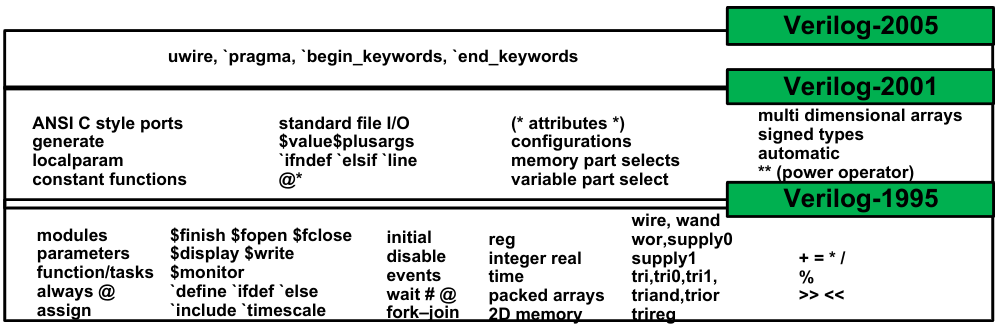
\includegraphics[width=0.98\textwidth]{img/01_ver.png}
\end{figure}

\end{frame}

%%%%%%%%%%%%%%%%%%%%%%%%%%%%%%%%%%%%%%%%%%%%%%%%%%%%%%%%%%%%
\begin{frame}
\frametitle{Module Review}

\begin{itemize}
\item What is an HDL?
\item How is the HDL description independent of the product implementation and why is this a good thing?
\item What level of abstractions is used in?
\begin{enumerate}
	\item Testbenches?
	\item Sythesizable designs?
	\item Netlists?
\end{enumerate}
\end{itemize}
\end{frame}

%%%%%%%%%%%%%%%%%%%%%%%%%%%%%%%%%%%%%%%%%%%%%%%%%%%%%%%%%%%%
\begin{frame}
\frametitle{Module Review Solutions}

\begin{itemize}
\item What is an HDL?
\begin{itemize}
	\item An HDL is a programming language with special constructs for modeling hardware, such as abstractions, concurrent behavior, and timing.
\end{itemize}
\item How is the HDL description independent of the product implementation and why is this a good thing?
\begin{itemize}
	\item The HDL is standard and the synthesizable subset is standard. You specify the target technology upon synthesis.
\end{itemize}
\item What level of abstractions is used in?
\begin{enumerate}
	\item Testbenches? $\rightarrow$ Behavioral
	\item Sythesizable designs? $\rightarrow$ RTL
	\item Netlists? $\rightarrow$ Structural
\end{enumerate}
\end{itemize}
\end{frame}

%%%%%%%%%%%%%%%%%%%%%%%%%%%%%%%%%%%%%%%%%%%%%%%%%%%%%%%%%%%%
\begin{frame}
\frametitle{Lab}

Lab 2-1: Exploring the VeriRISC CPU design

\begin{itemize}
\item Becoming familiar with the lab model, which is RISC CPU design
\end{itemize}
\end{frame}

%%%%%%%%%%%%%%%%%%%%%%%%%%%%%%%%%%%%%%%%%%%%%%%%%%%%%%%%%%%%
\begin{frame}
\frametitle{Questions - 1}

Which one or more of these does a HDL describe?

\begin{itemize}
\item[$\square$] design timing estimates
\item[$\square$] design connectivity
\item[$\square$] design behavior
\item[$\square$] design physical implementation
\end{itemize}
\end{frame}

%%%%%%%%%%%%%%%%%%%%%%%%%%%%%%%%%%%%%%%%%%%%%%%%%%%%%%%%%%%%
\begin{frame}
\frametitle{Questions - 2}

The more detail in a gate-level design helps the simulator to simulate the design more quickly?

\begin{itemize}
\item[$\square$] True
\item[$\square$] False
\end{itemize}
\end{frame}

%%%%%%%%%%%%%%%%%%%%%%%%%%%%%%%%%%%%%%%%%%%%%%%%%%%%%%%%%%%%
\begin{frame}
\frametitle{Questions - 3}

Which one is primary advantage of using a HDL?

\begin{itemize}
\item[$\square$] An HDL defines the simulator user interface
\item[$\square$] An HDL allows a designer to abstractly capture the design intent
\item[$\square$] Coding HDL is identical to writing a software program
\end{itemize}
\end{frame}

%%%%%%%%%%%%%%%%%%%%%%%%%%%%%%%%%%%%%%%%%%%%%%%%%%%%%%%%%%%%
\begin{frame}
\frametitle{Questions Solutions - 1}

Which one or more of these does a HDL describe?

\begin{itemize}
\item[$\boxtimes$] design timing estimates
\item[$\boxtimes$] design connectivity
\item[$\boxtimes$] design behavior
\item[$\boxtimes$] design physical implementation
\end{itemize}
\end{frame}

%%%%%%%%%%%%%%%%%%%%%%%%%%%%%%%%%%%%%%%%%%%%%%%%%%%%%%%%%%%%
\begin{frame}
\frametitle{Questions Solutions - 2}

The more detail in a gate-level design helps the simulator to simulate the design more quickly?

\begin{itemize}
\item[$\square$] True
\item[$\boxtimes$] False
\end{itemize}
\end{frame}

%%%%%%%%%%%%%%%%%%%%%%%%%%%%%%%%%%%%%%%%%%%%%%%%%%%%%%%%%%%%
\begin{frame}
\frametitle{Questions Solutions - 3}

Which one is primary advantage of using a HDL?

\begin{itemize}
\item[$\square$] An HDL defines the simulator user interface
\item[$\boxtimes$] An HDL allows a designer to abstractly capture the design intent
\item[$\square$] Coding HDL is identical to writing a software program
\end{itemize}
\end{frame}

\end{document}
